\chapter{Mengenal Kecerdasan Buatan dan Scikit-Learn}

\section{Kecerdasan Buatan}
\subsection{Definisi Kecerdasan Buatan}
\par
Kecerdasan buatan atau Artificial Intelligence merupakan kecerdasan/pengetahuan yang dimodelkan dan diajarkan ke mesin agar mesin tersebut memiliki kecerdasan yang sama seperti manusia sehingga dapat membantu pekerjaan yang umumnya dilakukan oleh manusia. Untuk memiliki kecerdasan serta mengupgrade skill dari AI nya sendiri, mesin membutuhkan data untuk menambah ilmu dan pengetahuan yang dimilikinya. Adapun proses belajar AI terdiri dari learning, reasoning, dan self-correction. Jadi tidak hanya diajari oleh manusia tetapi AI akan belajar sendiri berdasarkan pengalaman ia digunakan.
\subsection{Sejarah dan Perkembangan AI}
\par
Konsep AI sendiri sebenarnya sudah ada sejak zaman yunani kuno dan berkembang pada abad pertengahan 20. Dimulai dengan sosok John McCarthy yang disebut juga sebagai "bapak AI" merupakan seorang ilmuwan yang memiliki andil besar dalam perkembangan AI. Ia mendirikan dua buah lembaga penelitian yang bergerak di bidang AI, yaitu Stanford Artificial Intelligence Laboratory dan MIT Artificial Intelligence Laboratory. Selain itu, McCarthy juga turut mengajar di dua universitas yang memiliki nama di tingkat internasional tersebut. Disanalah, McCarthy mulai mengembangkan berbagai inovasi AI di berbagai bidang misalnya human skill, vision, listening, reasoning, dan movement of limbs. McCarthy juga menciptakan sebuah bahasa pemrograman yang disebut dengan LISP dan program yang bernama programs with common sense. Di dalam program tersebut terdapat teknologi yang berfungsi sebagai resolve atau pemecah suatu masalah.  
\par
Tahun 1959, Nathaniel Rochester dan separuh dari mahasiswanya menciptakan sebuah program yang memiliki teknologi menciptakan suatu teorema dengan menggunakan pernyataan-pernyataan yang tersedia, program ini juga disebut dengan Gheometry Theorm Prover.
\par
Perkembangan AI sempat melambat dan kembali berkembang lagi sekitar tahun 1980-an. Itu dimulai dengan penemuan sebuah sistem yang dinamakan R1 yang dapat melakukan konfigurasi pada komputer baru. Sistem ini ditemukan oleh Digital Equipment Corporation (DEC) yang selanjutnya pada tahun 1981, mereka telah menjalankan 40 sistem tersebut.
\par
Pada tahun yang sama, hampir semua perusahaan di Amerika memiliki divisi di bidang AI tersendiri sehingga sebagian besar terdapat kenaikan signifikan pada pendapatan perusahaan per-tahunnya.
\par
Untuk perkembangan AI di Indonesia sendiri sudah cukup banyak tetapi belum ada ilmuwan yang membuat teknologi sampai diakui oleh dunia. Salah satu contoh generasi muda yang melakukan inovasi dan terobosan teknologi pada bidang ini adalah Digital Native. Tidak hanya di bidang teknologi, mereka mencampurkan dan membuat sinergi antara teknologi, unsur seni, dan juga unsur alam.

\section{Machine Learning}
\subsection{Supervised Learning}
\par
Supervised Learning merupakan salah satu dari contoh aplikasi atau penerapan machine learning yang dikategorikan berdasarkan label. Yang dimaksud label disini adalah target variabel ada atau tidak data tersebut. Pada supervised learning, supervise disini dimaksud dengan label di tiap datanya. Label dimaksud dengan tag suatu data yang ditambahkan dalam machine learning.
\par
Algoritma yang digunakan pada Supervised Learning adalah :
\begin{enumerate}
    \item Klasifikasi dan Regresi
    \par Contoh cara kerja dari supervised learning adalah gambar kupu-kupu di tag "kupu-kupu" di tiap gambarnya, gambar burung di tag "burung" di tiap masing-masing imagenya. Karena ini termasuk machine learning kategori, maka mempunyai klasifikasinya sendiri misalnya (kupu-kupu, burung, dll.)
    \par
    Regresinya sendiri contoh (berat badan, tinggi badan, bentuk mata, bentuk mulut/parah, antena, dll.)
    \item Logistic Regression
    \item Model Ensemble
    \item Time Series
\end{enumerate}
\subsection{Unsupervised Learning}
\par
Unsupervised Learning memiliki beberapa keunggulan dibandingkan dengan Supervised Learning. Ia tidak menggunakan label dalam memprediksi variabel tetapi melihat kesamaan atas atribut-atribut yang dimiliki oleh variabel. Jika atribut-atribut yang diperiksa memiliki kemiripan maka akan dikelompokkan (clustering).
\par
Algoritma yang digunakan pada Unsupervised Learning adalah :
\begin{enumerate}
    \item Clustering
    \item Anomaly Detection
    \item Training Model
    \item Association Discovery
\end{enumerate}

\section{Data Set, Training Set, dan Testing Set}
\subsection{Data Set}
\par
Yang dimaksud dengan data set adalah data yang berfungsi untuk dipelajari/dilampaui oleh machine learning untuk mencapai tujuannya. Data Set ini terbagi lagi menjadi dua jenis tergantung fungsinya.
\subsection{Training Set}
\par
Merupakan data set yang digunakan untuk mencapai goal dari machine learning. Nantinya akan digunakan untuk membuat model suatu machine learning.
\subsection{Testing Set}
\par
Merupakan data set yang akan dicapai atau dilampaui, ini akan digunakan sebagai uji performa dalam model machine learning.
Membuat file main.py dan mengisinya dengan script contoh python penggunaan selenium(minimal 20 baris) yang melibatkan inputan user, kemudian mencoba untuk mengatasi error identasi.

\section{Instalasi}
\begin{enumerate}
    \item Instalasi library scikit dari anaconda, mencoba kompilasi dan uji coba ambil
contoh kode dan lihat variabel explorer
    \begin{figure}[!htbp]
    \centering
    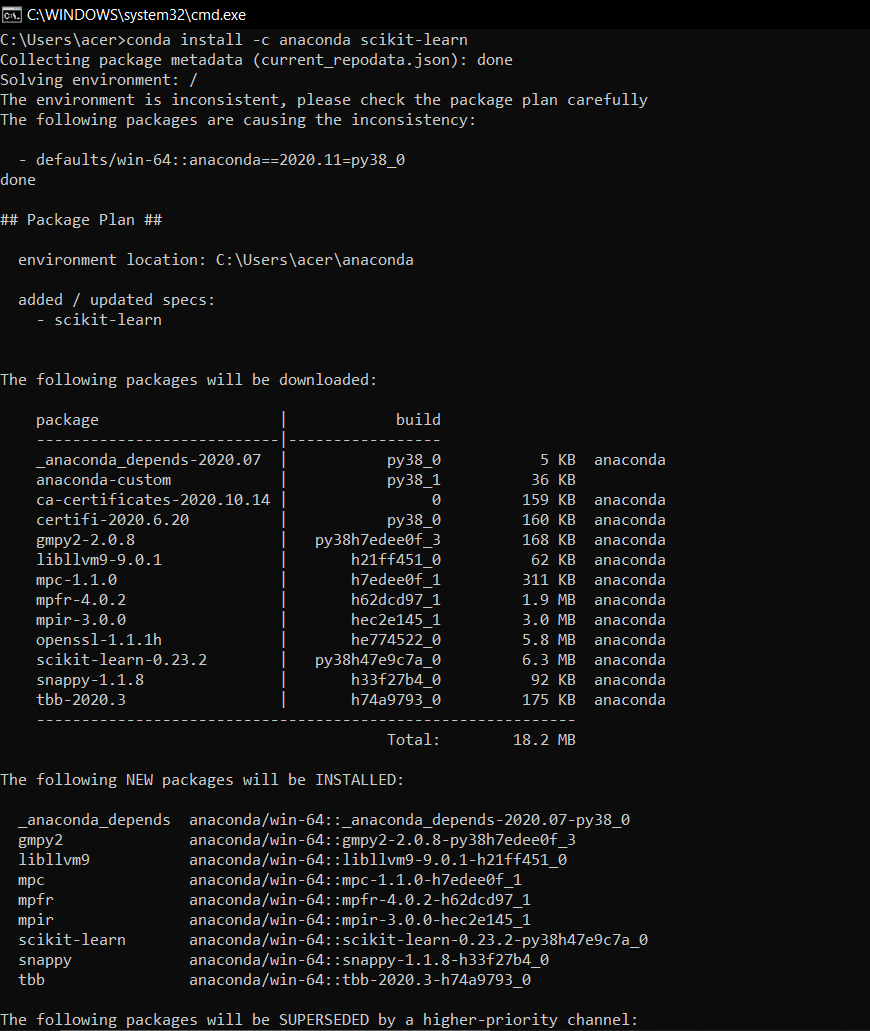
\includegraphics[scale=0.6]{figures/1.PNG}
    \caption{\textit{Install Library Scikit}}
    \label{Figure}
    \end{figure}
    \newpage
    \item Mencoba Loading an example dataset
    \begin{figure}[!htbp]
    \centering
    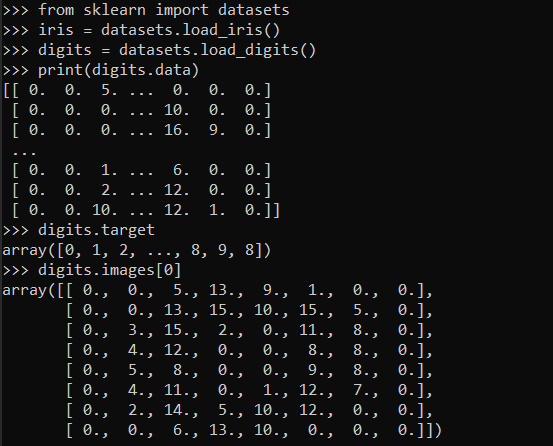
\includegraphics[scale=1]{figures/Loadingdatasets/1.PNG}
    \label{Figure}
    \end{figure}
    \par
    Penjelasan : 
    \par
    Baris ke-1, loading package yang akan digunakan;
    \par
    Baris ke-2, membuat variabel bernama iris yang isinya adalah fungsi load dataset iris. Dataset ini sudah tersedia default dari sklearn, ia berisikan 3 macam spesies bunga serta ukuran sepal dan petalnya;
    \par
    Baris ke-3, pada variabel digits akan dimuat dataset digit;
    \par
    Baris ke-4, display atau menampilkan data dari var digits;
    \par
    Baris ke-5-11 merupakan output dari digits.data;
    \par
    Baris ke-12, memuat/menampilkan fungsi target dari digits yang berisikan label;
    \par
    Baris ke-13 berisi output dari digits.target;
    \par
    Baris ke-14 Setiap slot dalam array sesuai dengan piksel, dan nilai dalam slot adalah; jumlah hitam dalam pixel
    \par
    Baris ke-15-22, output dari digits.images[0]
    \newpage
    \begin{figure}[!htbp]
    \centering
    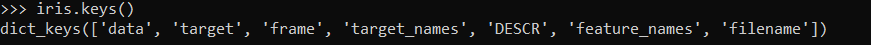
\includegraphics[scale=0.8]{figures/Loadingdatasets/5.PNG}
    \label{Figure}
    \end{figure}
    \par
    Penjelasan :
    \par
    Baris ke-1, menampilkan seluruh keys dalam dataset iris untuk mengetahui apa saja yang berada dalam dataset tersebut; 
    \par
    Baris ke-2, Ouput yang berupa daftar dari keys atau kata kunci yang terdapat dalam dictionary
    \begin{figure}[!htbp]
    \centering
    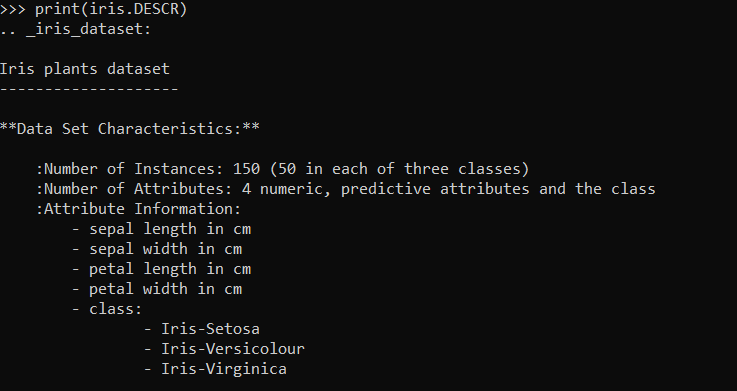
\includegraphics[scale=0.9]{figures/Loadingdatasets/6.PNG}
    \label{Figure}
    \end{figure}
    \par
    Penjelasan :
    \par
    Baris ke-1, Terdapat salah satu key DESCR pada dataset iris, dengan fungsi ini kita akan menampilkan deskripsi dari dataset;
    \par
    Baris ke-2 dst., merupakan output yang berisi deskripsi dataset iris. Dapat diketahui ia memiliki 4 atribut numerik yaitu : sepal length, sepal width, petal length, dan petal width. Selain itu ia memiliki 3 jenis spesies (class) yaitu : Iris Setosa, Iris-Versicolour, dan Iris-Virginica.
    \newpage
    \item Mencoba Learning and predicting
    \begin{figure}[!htbp]
    \centering
    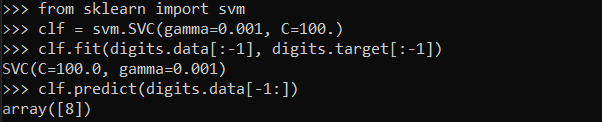
\includegraphics[scale=1]{figures/Learningandpredict/1.PNG}
    \label{Figure}
    \end{figure}
    \par
    Baris ke-1, dari library sklearn import module svm (Support Vector Machine) / Algoritma Klasifikasi
    \par
    Baris ke-2, membuat variabel clf yang didalamnya memuat definisi dari fungsi SVC pada module svm yang telah diimport di awal
    \par
    Baris ke-3, menjalankan fungsi fit dari variabel clf
    \par
    Baris ke-4, output clf.fit
    \par
    Baris ke-5, menjalankan fungsi predict/prediksi dari var clf
    \par
    Baris ke-6, output clf.predict
    \item Mencoba Model persistence
    \par
    Setelah dilatih, model diharapkan untuk dapat mempertahankan model tersebut tanpa perlu dilatih kembali di masa depan. 
    \begin{figure}[!htbp]
    \centering
    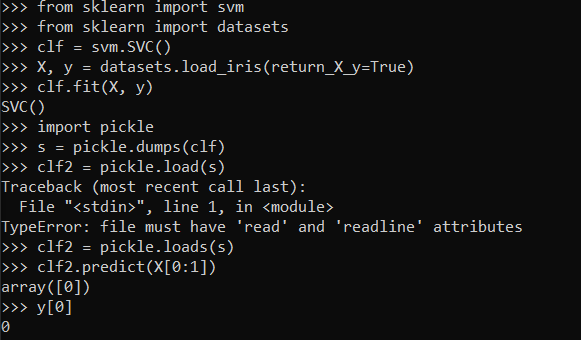
\includegraphics[scale=1]{figures/Modelpersistence/1.PNG}   \label{Figure}
    \end{figure}
    \newpage
    \par
    Dalam beberapa kasus, lebih baik menggunakan joblib replacement dari pickle
    \begin{figure}[!htbp]
    \centering
    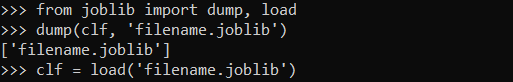
\includegraphics[scale=1]{figures/Modelpersistence/2.PNG}   \label{Figure}
    \end{figure}
    \item Mencoba Conventions
    \par
    Pada conventions sendiri, diterapkan peraturan khusus agar perilaku lebih prediktif (ketika melakukan prediksi).
    \begin{itemize}
        \item Type Casting
        \begin{figure}[!htbp]
        \centering
        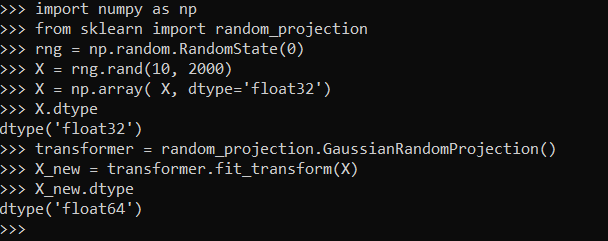
\includegraphics[scale=1]{figures/Conventions/8.PNG}
        \label{Figure}
        \end{figure}
        \item Refitting and updating parameters
        \begin{figure}[!htbp]
        \centering
        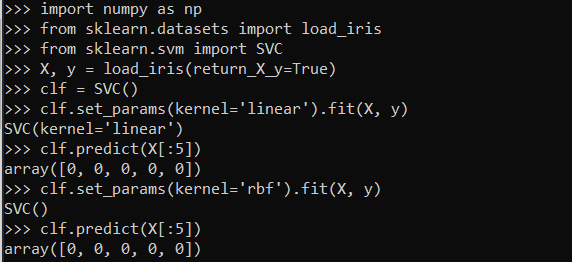
\includegraphics[scale=1]{figures/Conventions/10.PNG}
        \label{Figure}
        \end{figure}
        \newpage
        \item Multiclass vs multilabel fitting
         \begin{figure}[!htbp]
        \centering
        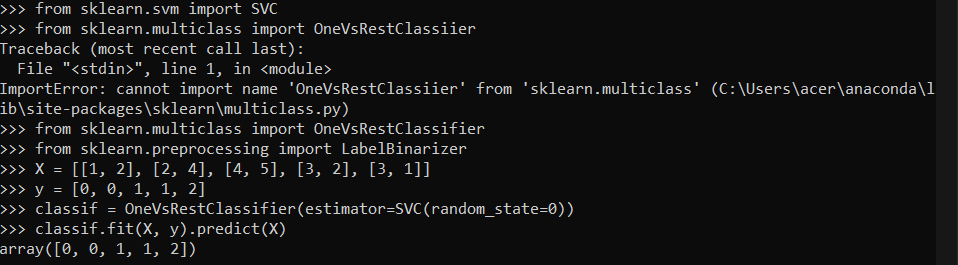
\includegraphics[scale=0.7]{figures/Conventions/11.PNG}
        \label{Figure}
        \end{figure}
        \par
        Pada kasus di atas lebih cocok untuk pengklasifikasian 1d array, sedangkan untuk 2d array :
         \begin{figure}[!htbp]
        \centering
        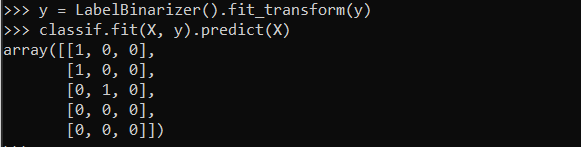
\includegraphics[scale=1]{figures/Conventions/12.PNG}
        \label{Figure}
        \end{figure}
        \par
        Pada kasus lainnya, pengklasifikasi cocok-cocok saja dengan berbagai macam contoh yang pada masing-masingnya memiliki multilable
        \begin{figure}[!htbp]
        \centering
        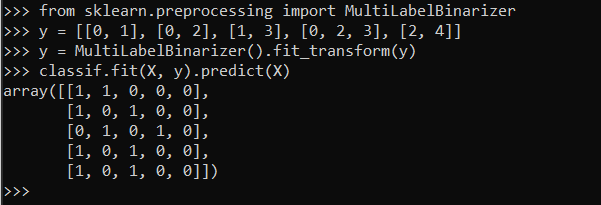
\includegraphics[scale=1]{figures/Conventions/13.PNG}
        \label{Figure}
        \end{figure}
        \par
    \end{itemize}
\end{enumerate}
\section{ Penanganan Error}
\par
Dari percobaan yang dilakukan di atas, apabila mendapatkan error maka:
\begin{enumerate}
    \item skrinsut error[hari ke 2](10)
    \item Tuliskan kode eror dan jenis errornya [hari ke 2](10)
    \item Solusi pemecahan masalah error tersebut[hari ke 2](10)
\end{enumerate}
